\documentclass[letters,usenatbib,useAMS]{mnras}

\usepackage{amsmath,amssymb}
\usepackage{graphicx}
\usepackage[T1]{fontenc}
\usepackage{booktabs}

\title[GMaster: difference-form GPU MASTER]{GMaster: a difference-form Wigner-$d$ march for GPU MASTER estimation}

\author[Xu]{
Licong Xu$^{1}$\thanks{E-mail: lx256@cam.ac.uk}\\
$^{1}$Institute of Astronomy, University of Cambridge, Madingley Road, Cambridge CB3 0HA, UK
}

\date{Accepted XXX. Received YYY; in original form ZZZ}
\pubyear{2026}

\begin{document}
\label{firstpage}
\pagerange{\pageref{firstpage}--\pageref{lastpage}}
\maketitle

\begin{abstract}
The latitudinal factor of a HEALPix spherical-harmonic transform is a three-term Jacobi recurrence in $\ell$ for each order $m$. In float32 that recurrence is unstable near the poles and at every turning point: the characteristic roots collide, and a rounding of size $u\lvert v\rvert$ is amplified by $1/\sin\phi$. We rewrite the march so that the carried pair is $(v_n,D_n)$ with $D_n=v_n-v_{n-1}$ rather than $(v_n,v_{n-1})$. The difference coefficient vanishes as $\phi^2$ exactly where the plain form is ill-conditioned, error is injected at the scale of $D\sim\phi\,v$, and the float32 floor becomes the random walk $\sqrt{n}\,u$. Against the float64 recurrence at $N_{\mathrm{side}}=1024$ the maximum relative error over every lane falls from $4.2\times10^{-2}$ (plain) to $2.8\times10^{-6}$ (shipped). The identities of the rewrite, a southern-hemisphere reflection onto the same code path, and an exact per-block power-of-two rescale are proved in Lean~4. The kernel is CUDA, called from JAX through the XLA FFI, and is the default latitudinal operator in GMaster, a GPU library with the public API of NaMaster. On one RTX~PRO~6000 Blackwell against NaMaster on a 96-core Threadripper~PRO~9995WX the end-to-end MASTER pipeline is $10$--$21\times$ faster at $N_{\mathrm{side}}=128$--$2048$ in both spins, with coupled spectra agreeing to $1.2\times10^{-7}$--$1.2\times10^{-5}$. On the ACT DR6 night PA4 $f150$ coadd and a FLAMINGO L2p8 Compton-$y$ map, both at $N_{\mathrm{side}}=4096$, warm wall-clock is $7.6$--$8.6\,\mathrm{s}$ against $70\,\mathrm{s}$ for NaMaster, with fractional bandpower rms $1.4\times10^{-5}$ and $2.3\times10^{-7}$. No other GPU spherical-harmonic code was timed.
\end{abstract}

\begin{keywords}
methods: numerical -- cosmology: cosmic microwave background -- cosmology: large-scale structure of Universe
\end{keywords}

\section{Introduction}

The MASTER estimator \citep{hivon2002} recovers binned angular power spectra from masked spherical maps by analysing the masked fields, forming coupled pseudo-spectra, building a mode-coupling matrix from the mask, and decoupling. NaMaster \citep{alonso2019} is the CPU reference. Its transforms run through DUCC, the successor of libsharp \citep{reinecke2013}, on the HEALPix pixelisation \citep{gorski2005}. The coupling algebra has a structured Wigner-$3j$ recurrence \citep{kiddier2026}.

On a GPU the same two cubic stages remain. An on-the-fly associated-Legendre recurrence, as in SHTns \citep{schaeffer2013} and DUCC, is a serial chain in $\ell$ with a reduction over colatitude at every degree. That pattern matches AVX-512 CPUs and mismatches GPU SIMT. A precomputed Legendre matrix, as in the precompute mode of s2fft \citep{price2024}, inverts the bottleneck provided the table fits. Related GPU work \citep{belkner2024,reinecke2023} retains an on-the-fly latitudinal factor and is not a drop-in for a full-sky HEALPix MASTER pipeline.

GMaster is a JAX implementation of the NaMaster public API. This Letter isolates one change that made a table-free float32 latitudinal kernel accurate enough to be the default at every $N_{\mathrm{side}}\ge64$: marching the difference pair of the Jacobi row attached to $d^\ell_{m,-s}(\theta)$ rather than the consecutive values. The recurrence, a reflection that sends the southern hemisphere through the same instructions, and the exactness of a per-block power-of-two rescale are proved in Lean~4 \citep{demoura2021,mathlib2020}. We report the end-to-end MASTER board and two real-map overlays. This is not a cosmological analysis: no beam, split cross-spectrum, or covariance is applied to the survey maps.

\section{Difference-form march}

Every Wigner function $d^\ell_{m,-s}(\theta)$ is an algebraic multiple of a Jacobi polynomial \citep[NIST DLMF 14.9.16, 18.3]{olver2010},
\begin{equation}
\begin{split}
  d^\ell_{m,-s}(\theta)
  &= (-1)^m\,2^{\varepsilon_m\mathrm{LG2N}}\\
  &\quad\times
    \Bigl(\sin\tfrac{\theta}{2}\Bigr)^\alpha
    \Bigl(\cos\tfrac{\theta}{2}\Bigr)^\beta
    P_n^{(\alpha,\beta)}(\cos\theta),
\end{split}
\end{equation}
with $\alpha=m+s$, $\beta=\lvert m-s\rvert$, $n=\ell-\max(m,s)$ and $\mathrm{LG2N}=\log_2\sqrt{(\ell+m)!(\ell-m)!/((\ell-s)!(\ell+s)!)}$. The family obeys a three-term recurrence in $n$ \citep[DLMF 18.9.1]{olver2010}. Writing $x=\cos\theta$ and $v_n$ for the marched polynomial,
\begin{equation}
\label{eq:jacobi}
  v_n = A_n v_{n-1}-B_n v_{n-2},\qquad A_n=c_1 x+c_0,\quad B_n=c_2,
\end{equation}
where $c_1,c_0,c_2$ depend only on $(\ell,m)$. A float64 march of~\eqref{eq:jacobi} agrees with a numpy oracle of the same coefficients to $1.5\times10^{-15}$ at $N_{\mathrm{side}}=1024$. Plain float32 of the same recurrence reaches a maximum relative error of $4.2\times10^{-2}$ over the row (Table~\ref{tab:dform}).

Over a few degrees the coefficients are nearly constant and $c_2\to1$, so the row is locally $v_n\approx A v_{n-1}-v_{n-2}$ with characteristic roots $e^{\pm i\phi}$ and $2\sqrt{c_2}\cos\phi=A$. In the oscillatory region $\lvert A\rvert<2$, and $\phi\to0$ both at the poles and at every turning point $m\approx(\ell+\tfrac12)\sin\theta$. A rounding $\delta\sim 2u\lvert v\rvert$ of $\mathrm{fl}(Av_{k-1}-Bv_{k-2})$ perturbs the state by $(\delta,0)$, which decomposes on the modes $(e^{\pm i\phi},1)$ with amplitude $\delta/(2\sin\phi)$ each and evolves as $\delta\sin((n-k+1)\phi)/\sin\phi$: every rounding is amplified by $1/\sin\phi$, and over $n$ steps with random signs the relative error is $\sim\sqrt{n}\,u/\sin\phi$. On the first HEALPix ring at $N_{\mathrm{side}}=4096$, $\theta\approx2\times10^{-4}$ and $1/\sin\phi\approx5\times10^3$, giving a floor of a few per cent, the order of the plain-float32 row of Table~\ref{tab:dform}. A systematic error is worse: a relative error $\epsilon$ in $x$ perturbs $A$ at every step, and $2\cos\phi=A$ turns it into a coherent phase drift $\sim n\,c_1x\,\epsilon/(2\sin\phi)$, of order a radian at $n=12288$ for $\epsilon=u$.

Let $D_n=v_n-v_{n-1}$. Then for $n\ge2$
\begin{equation}
\label{eq:diff}
  D_n=(A_n-1-B_n)\,v_{n-1}+B_n D_{n-1},\qquad v_n=v_{n-1}+D_n.
\end{equation}
In terms of $\phi$, the difference coefficient is $C=A-1-c_2\approx-\phi^2$, so $D\approx\phi\,\lvert v\rvert$ exactly where the plain march is ill-conditioned. A rounding of $v\leftarrow\mathrm{fl}(v+D)$ lands on $v$ with $D$ fixed and is not amplified. A rounding of $D\leftarrow\mathrm{fl}(c_2 D+C v)$ lands on $D$ at scale $u\phi\lvert v\rvert$ and, after the $1/(2\sin\phi)$ modal factor, contributes $O(u\lvert v\rvert)$ per step. Both kinds therefore give a random-walk floor $\sqrt{n}\,u$ independent of $\phi$: $\sqrt{3072}\,u\approx3.3\times10^{-6}$ at $N_{\mathrm{side}}=1024$, against the measured $2.8\times10^{-6}$.

The only coefficient on the amplified path is $C$, and the argument needs its error to be $O(u\lvert C\rvert)$, not $O(u\lvert A\rvert)$. Writing $C_n=c_1(x-1)+E_n$ with $E_n=c_1-1-c_2+c_0$, the kernel carries $x-1$ rather than $x$: near a pole $x-1\sim-\theta^2/2$, so a single-word $x$ would inject a relative error $u/(\theta^2/2)$ into the leading term of $C$, and a single-word $E$ would leave an error $\sim u\lvert c_1\rvert$ that does not shrink with $C$. Both are systematic and drift the phase. The kernel therefore stores $\lvert x\rvert-1=x_h+x_l$, $c_1=c_{1h}+c_{1l}$ and $E=E_h+E_l$ as float32 pairs, each split from float64 to $2^{-48}$ \citep{dekker1971}, and forms
\begin{equation}
\label{eq:Cfma}
  C=\mathrm{fma}(c_{1h},x_h,E_h)+\bigl[\mathrm{fma}(c_{1h},x_l,\mathrm{fma}(c_{1l},x_h,E_l))\bigr].
\end{equation}
The first \texttt{fma} rounds once, by $u\lvert C\rvert$, and that rounding vanishes with $C$ at the turning point where the amplification peaks; the bracket is $\sim2^{-24}$ of the leading terms. A single-word $C$ leaves the coherent $u\lvert c_1\rvert$-class drift, growing like $n$ rather than $\sqrt n$: the $4\times10^{-5}$ floor in the middle row of Table~\ref{tab:dform}. The coefficient $c_2$ is single-word, because its error enters as $u\lvert D\rvert\sim u\phi\lvert v\rvert$ on $D$, the unamplified kind.

The southern hemisphere needs no second code path. If $v_n=(c_1x+c_0)v_{n-1}-c_2v_{n-2}$ then $w_n:=(-1)^nv_n$ satisfies
\begin{equation}
\label{eq:refl}
  w_n=\bigl(c_1(-x)-c_0\bigr)w_{n-1}-c_2w_{n-2},
\end{equation}
the same recurrence with $y=\lvert x\rvert$ for $x$ and $-c_0$ for $c_0$, whose difference coefficient is $c_1(y-1)+E^-_n$ with $E^-_n=c_1-1-c_2-c_0$. Every lane, northern or southern, therefore marches $\lvert x\rvert-1\in(-1,0]$ with the same instructions and one of two table columns $E^\pm$, and the emit restores the sign on odd $n$. Each lane stores $v\cdot2^{ex}$ with $ex$ an integer and is rescaled by an exact power of two every eight degrees; the map $(v,D)\mapsto(v+D',D')$ is linear, so the represented value is unchanged, and the per-degree growth is bounded by $1+\lvert C\rvert+c_2\le2^{15}$, so eight degrees cannot overflow. The emit factorises the Jacobi normalisation $2^{\varepsilon_m\mathrm{LG2N}}$ into a per-lane power of two and a per-degree mantissa proved to lie in $[2^{-45.5},2)$, so no exponent lane leaves the kernel. Equations~\eqref{eq:diff} and~\eqref{eq:refl}, the seeds, the homogeneity of the rescale, and the range of the mantissa are theorems in a Lean~4 development on Mathlib that builds with no \texttt{sorry}; the modal error argument is not formalised, and is checked by Table~\ref{tab:dform}.

\begin{table}
\centering
\caption{Maximum relative error of a float32 march against the float64 recurrence, over every lane, at $N_{\mathrm{side}}=1024$ spin~$0$. The two-word row is the shipped kernel ($5.7\times10^{-6}$ at $N_{\mathrm{side}}=4096$).}
\label{tab:dform}
\footnotesize
\setlength{\tabcolsep}{3pt}
\begin{tabular}{@{}lccc@{}}
\toprule
Float32 march & $m=0$ & $m=1000$ & $m=L/2$ \\
\midrule
Plain, single word          & $4.2\times10^{-2}$ & $8.8\times10^{-5}$ & $3.1\times10^{-5}$ \\
Difference form, 1-word $C$ & $4.1\times10^{-5}$ & $8.6\times10^{-5}$ & $5.1\times10^{-5}$ \\
Difference form, 2-word $C$ & $2.8\times10^{-6}$ & $2.9\times10^{-6}$ & $1.6\times10^{-5}$ \\
\bottomrule
\end{tabular}
\end{table}

The kernel is CUDA, one warp per $(m$, ring tile), exposed as XLA FFI handlers inside \texttt{jit}. A field and its mask are two transforms of the same rows: the analysis kernel takes both as emit channels, so an \texttt{NmtField} is not two launches. For $s=0$ the southern hemisphere is folded into the northern recurrence. The default at $L=\ell_{\max}+1\ge192$ ($N_{\mathrm{side}}\ge64$) is this march; an exact float64 route remains available by flag. The difference-form $D_n$ march is not GPU-intrinsic; only the shipped latitudinal operator is CUDA. A fair CPU timing of the same algorithm requires porting that kernel, not the JAX CPU fallback with the CUDA path gated out.

\section{Performance}

\begin{figure*}
\centering
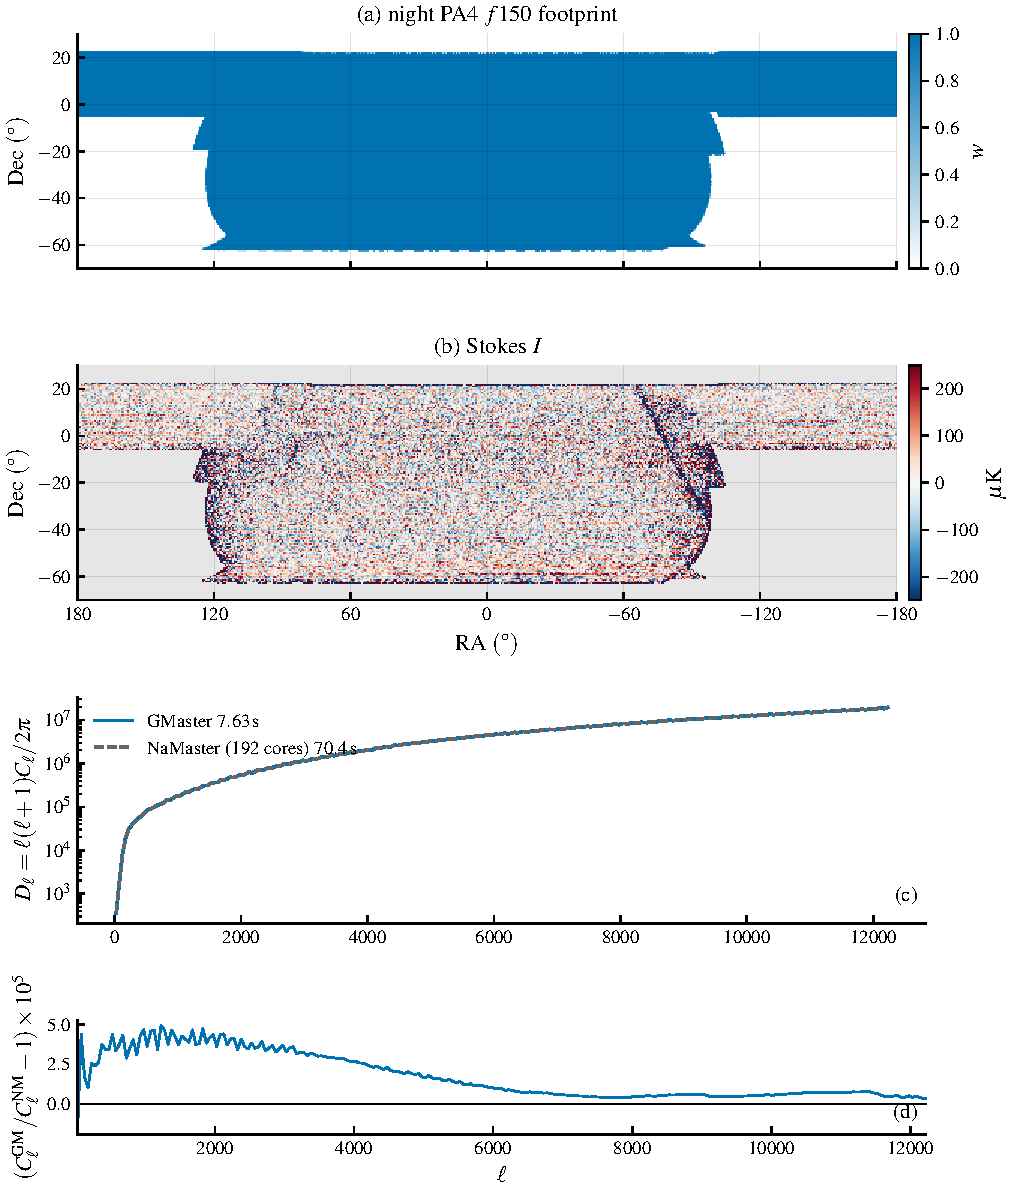
\includegraphics[width=0.78\textwidth]{figures/fig_act_overlay.pdf}
\caption{ACT DR6 night PA4 $f150$ source-free coadd \citep{naess2025} at $N_{\mathrm{side}}=4096$. (a)~Survey window used as the mask ($f_{\mathrm{sky}}=0.481$). (b)~Stokes $I$ on that footprint. (c)~Decoupled TT $D_\ell$ from GMaster and NaMaster, linear bins of width $50$, $n_{\mathrm{iter}}=3$. (d)~Fractional difference. This is a methods overlay, not an ACT science product.}
\label{fig:act}
\end{figure*}

All timings are single-tenant on one NVIDIA RTX~PRO~6000 Blackwell. The CPU reference is NaMaster~3.0 / \texttt{ducc0}~0.39.1 on the same host, a 96-core Threadripper~PRO~9995WX. End-to-end totals are warmed medians of field construction, coupling matrix, coupled cell and decoupling. Relative error is the maximum relative deviation of the coupled spectrum from \texttt{pymaster}. Isolated transforms are timed against the \texttt{ducc0} call NaMaster issues.

Table~\ref{tab:e2e} is the MASTER board. The shipped route is $10.2$--$21.2\times$ NaMaster at $N_{\mathrm{side}}=128$--$2048$ in both spins, $5.0$--$5.8\times$ at $N_{\mathrm{side}}=64$ (launch-latency bound) and $9.6\times$ at $N_{\mathrm{side}}=4096$ spin~$0$. Stock NaMaster segfaults at $N_{\mathrm{side}}=4096$ spin~$2$ on 32-bit coupling-matrix indices; GMaster finishes that cell in $8.8\,\mathrm{s}$. One isolated latitudinal pass against \texttt{ducc0} is $5.6$--$8.5\times$ at $N_{\mathrm{side}}=1024$--$4096$, with coefficient agreement $\sim1.2\times10^{-7}$. With the march disabled and rings and coupling forced to float64, decoupled bandpowers reproduce $4.8\times10^{-13}$ at $N_{\mathrm{side}}=256$ spin~$0$. The shipped default is a float32-class route: $\sim10^{-6}$ relative on the decoupled $C_\ell$, five to six orders below NaMaster's own $n_{\mathrm{iter}}=3$ truncation.

\begin{table}
\centering
\caption{End-to-end MASTER on the 96-core host. NM and GM are NaMaster and GMaster milliseconds. rel is the maximum relative deviation of the coupled spectrum from \texttt{pymaster}.}
\label{tab:e2e}
\footnotesize
\setlength{\tabcolsep}{3.5pt}
\begin{tabular}{@{}rrrrrl@{}}
\toprule
$N_{\mathrm{side}}$ & spin & NM & GM & Ratio & rel \\
\midrule
64   & 0 & $9$     & $2$    & $5.8$  & $1.15\times10^{-7}$ \\
64   & 2 & $12$    & $2$    & $5.0$  & $2.72\times10^{-7}$ \\
128  & 0 & $20$    & $1$    & $13.3$ & $4.92\times10^{-7}$ \\
128  & 2 & $40$    & $3$    & $13.1$ & $4.37\times10^{-7}$ \\
256  & 0 & $58$    & $4$    & $15.0$ & $6.36\times10^{-7}$ \\
256  & 2 & $161$   & $8$    & $20.7$ & $6.30\times10^{-7}$ \\
512  & 0 & $314$   & $17$   & $18.1$ & $7.07\times10^{-7}$ \\
512  & 2 & $641$   & $30$   & $21.2$ & $2.99\times10^{-6}$ \\
1024 & 0 & $1682$  & $102$  & $16.5$ & $1.45\times10^{-6}$ \\
1024 & 2 & $3017$  & $212$  & $14.2$ & $7.79\times10^{-6}$ \\
2048 & 0 & $10311$ & $1014$ & $10.2$ & $7.25\times10^{-6}$ \\
2048 & 2 & $17767$ & $1244$ & $14.3$ & $1.19\times10^{-5}$ \\
4096 & 0 & $71583$ & $7458$ & $9.6$  & $7.0\times10^{-6}$ \\
4096 & 2 & ---     & $8805$ & ---    & finite \\
\bottomrule
\end{tabular}
\end{table}

Figure~\ref{fig:act} is the same estimator on the ACT DR6 night PA4 $f150$ source-free coadd \citep{naess2025}, Stokes $I$, degraded from native $N_{\mathrm{side}}=8192$ to $4096$. The mask is the survey window (finite non-zero pixels; $f_{\mathrm{sky}}=0.481$). GMaster and NaMaster share the mask, linear bins of width $50$, and $n_{\mathrm{iter}}=3$. Decoupled TT agrees to $\mathrm{rms}(C_\ell^{\mathrm{GM}}/C_\ell^{\mathrm{NM}}-1)=1.41\times10^{-5}$. Wall-clock after compilation: $7.63\,\mathrm{s}$ versus $70.4\,\mathrm{s}$ on $192$ cores. The FLAMINGO L2p8 unlensed Compton-$y$ lightcone \citep{schaye2023}, full sky at $N_{\mathrm{side}}=4096$, gives rms $2.32\times10^{-7}$ in $8.64\,\mathrm{s}$ versus $69.5\,\mathrm{s}$. Both overlays time only the estimator. Figure~\ref{fig:accuracy} puts the float32 floors of Table~\ref{tab:dform} beside pipeline-level agreement of the shipped and exact routes, and Figure~\ref{fig:scoreboard} is the wall-clock board of Table~\ref{tab:e2e}.

\begin{figure}
\centering
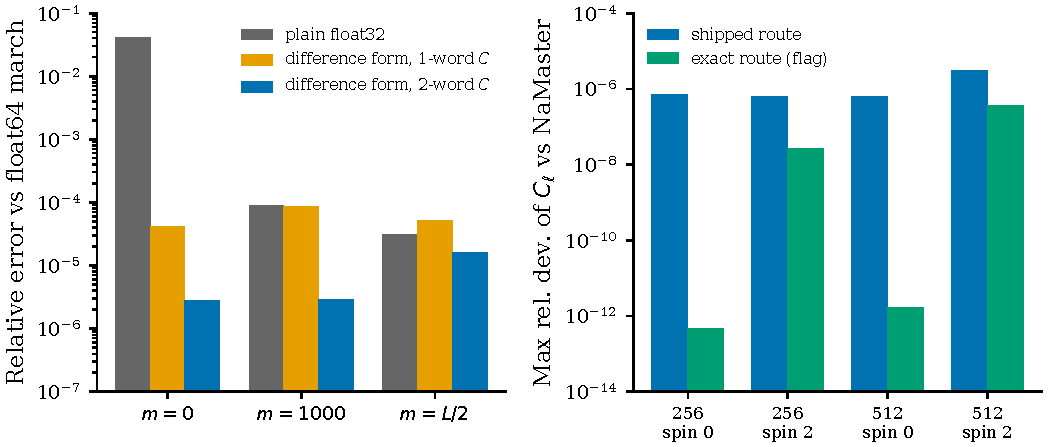
\includegraphics[width=\columnwidth]{figures/fig_accuracy.pdf}
\caption{Left: relative error of a float32 march against the float64 recurrence at $N_{\mathrm{side}}=1024$ spin~$0$. Right: maximum relative deviation of the decoupled bandpowers from NaMaster for the shipped route and the exact float64 route.}
\label{fig:accuracy}
\end{figure}

\begin{figure}
\centering
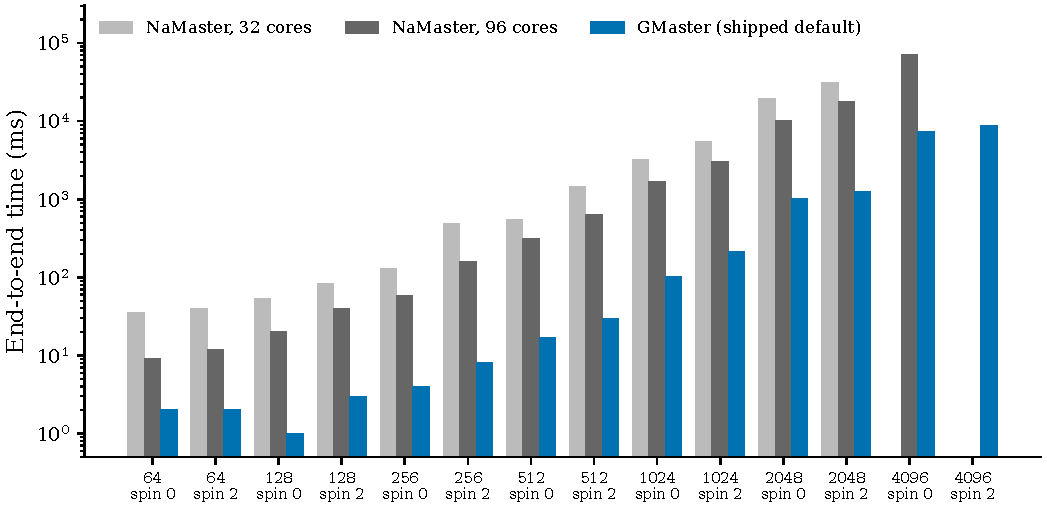
\includegraphics[width=\columnwidth]{figures/fig_scoreboard.pdf}
\caption{End-to-end MASTER wall time on the host of Table~\ref{tab:e2e}. Grey is NaMaster on 96 cores; blue is GMaster. NaMaster is absent at $N_{\mathrm{side}}=4096$ spin~$2$, where stock NaMaster segfaults on 32-bit coupling-matrix indices.}
\label{fig:scoreboard}
\end{figure}

\section{Conclusions}

A three-term Jacobi recurrence in float32 is limited by $1/\sin\phi$ amplification, not by the width of its words. Marching $(v,v-v_{\mathrm{prev}})$ moves the injection of every rounding onto a difference that already vanishes at the turning points, and a two-word $C$ removes the residual coherent drift. Carried as a CUDA kernel behind NaMaster's API, that rewrite is the default latitudinal operator in GMaster and is $10$--$21\times$ NaMaster at $N_{\mathrm{side}}=128$--$2048$ on the board of Table~\ref{tab:e2e}. The same pipeline on an ACT DR6 coadd and a FLAMINGO Compton-$y$ map at $N_{\mathrm{side}}=4096$ agrees at $10^{-5}$--$10^{-7}$ in under nine seconds.

No other GPU spherical-harmonic implementation was timed. The shipped default trades NaMaster's float64 contract for $\sim10^{-6}$ relative agreement; the exact route is one flag. The overlays are methods comparisons, not science products.

\section*{Acknowledgements}

NaMaster, DUCC/libsharp, s2fft, threej\_cosmo and SHTns are the reference stack against which the numbers were measured. The Lean~4 development uses Mathlib. ACT DR6 maps are those of \citet{naess2025}. Portions of the library and of this manuscript were drafted with coding assistants; every numerical claim was measured on the hardware of Section~3.

\section*{Data Availability}

GMaster, the overlay scripts, the committed bandpowers of both overlays and a notebook that rebuilds Figure~\ref{fig:act} and the timing table from them are at \url{https://github.com/licongxu/GMaster}. Figure~\ref{fig:act} uses the public ACT DR6 maps \citep{naess2025}. The FLAMINGO L2p8 Compton-$y$ lightcone is described by \citet{schaye2023}.

\bibliographystyle{mnras}
\bibliography{refs}

\bsp
\label{lastpage}
\end{document}
